\documentclass[conference]{IEEEtran}
\usepackage{fancyhdr}
\usepackage{graphicx}
\usepackage{listings}
\usepackage{xcolor}
\usepackage{amsmath}
\usepackage{hyperref}
\usepackage{indentfirst}
\usepackage{titlesec}
\usepackage{subcaption}
\setlength{\marginparwidth}{2cm}
\usepackage{todonotes}
\hypersetup{
    breaklinks=true,
    urlcolor=blue,
    linkcolor=black,
    citecolor=black
}

\lstset{
    language=C,
    basicstyle=\ttfamily\small,
    stringstyle=\color{red},
    commentstyle=\color{blue}{},
    breaklines=true
}

\titlespacing*{\section}
{0pt}                      % left margin
{2ex plus 1ex minus .2ex}  % space before
{1ex plus .2ex}            % space after

\titlespacing*{\subsection}
{0pt}
{3ex plus 1ex minus .2ex}
{0.8ex plus .2ex}

\title{Final Project Proposal: Analytical Placement Via FPGA}
\author{
    \IEEEauthorblockN{Parker Schless (pis7), Colin Muessig (cjm369), Jeremy Ku-Benjet (jk2582)}
    \IEEEauthorblockA{ECE 5760: Hardware Acceleration via FPGA \\
    Cornell University: School of Electrical and Computer Engineering}
}

\begin{document}
\maketitle

\section{Project Overview}
EDA algorithms for ASIC and FPGA design have historically been implemented as CPU-only workloads, with limited exploitation of multicore parallelism. In contrast, modern compute-intensive workloads in other domains routinely offload work to GPUs or dedicated accelerators, freeing the CPU to handle orchestration. Despite significant R\&D investment, major EDA vendors still rely predominantly on CPU-based implementations, owing to the complexity of their existing tool infrastructure and the difficulty of parallelizing algorithms whose core data structures are highly irregular. There has been recent work in academia using GPUs via machine learning frameworks to implement placement\cite{dreamplace}. We take some inspiration from this and propose using the Cyclone V FPGA on the DE1-SoC board to accelerate standard cell placement, a key EDA algorithm, by offloading its computational bottleneck to programmable logic. By writing a C baseline to run on the HPS as well as a Verilog accelerator targeting the FPGA fabric, we aim to explore the potential performance benefits of hardware acceleration for ASIC placement flows.

\section{Parts and Costs}
Our project does not require any additional parts other than the same FPGA board we have been using for the previous lab assignments.

\section{Societal Impact}
% A paragraph describing the standards (IEEE, ISO, ANSI, etc) relevant to your project.
% safety considerations (lasers?, wires connected to human?)
% human factors and usability
% interface design considerations for people with special needs (e.g. color blindness, sight resolution)
% Intellectual property considerations. (music clips?, code?, images?)
% If you use any RF transmitter, include compliance information with FCC regulations
% Other legal considerations such as FDA or motor vehicle codes.

The impact of this project is significant, since commercial tool flows do not widely use hardware acceleration for placement, if at all. By demonstrating a measurable speedup, we can show that using dedicated hardware to run these algorithms is a worthy problem to be researched in more detail. Additionally, faster placement runtimes would shorten iteration cycles, giving ASIC engineers more opportunities to explore design alternatives and potentially improve overall quality of results (QoR), rather than waiting for hours-long tool runs to complete before evaluating the effect of a minor change.

\section{Technology and Implementation}
% A block diagram or pseuocode
% Tentative source code (if you have it)
% A tentative schematic for any hardware you need to build.
% A parts list with specific parts types, so that we can see if we have the material.

\subsection{Background Information}

We demonstrate our goal of accelerating EDA algorithms using dedicated hardware through optimization of a modern placement algorithm known as analytical placement, described thoroughly in a survey by Chang et al.~\cite{chang2007analytical}, though there have been some more recent developments we will try to incorporate. At a high level, placement is the process by which each standard cell is assigned to a location on the chip die given an input netlist of synthesized gates. An analogous problem exists for FPGA logic element packing; however, in this project we focus on the ASIC standard-cell formulation. When performing placement, the algorithm must meet multiple objectives: minimizing some cost metric (normally total wirelength), preventing cells from overlapping, adhering to placement density constraints, and producing a routable placement. Earlier approaches such as simulated annealing and min-cut placement struggle with modern design scales: simulated annealing is too slow for millions of cells, while min-cut methods can lack global optimization quality due to their top-down, hierarchical nature~\cite{chang2007analytical}. As such, analytical placement is the modern solution to the placement optimization problem. It formulates placement as a mathematical programming problem with an objective function and constraint set, then uses analytical methods to optimize the objective.

The placement process first starts with the global placement step, where approximate positions of cells modeled as a hypergraph of vertices (cells) and hyperedges (nets) are determined by minimizing the objective function, which we choose as the common total wirelength metric, subject to cell non-overlap constraints. Exact design-rule compliance is deferred to later stages to keep this step tractable. Two key ingredients are required: a wirelength model and an overlap reduction technique.

The wirelength of the design is typically measured by the total half-perimeter wirelength (HPWL):

\[
W(V,E) = \sum_{e \in E} \left( L_{e,x} + L_{e,y} \right)
\]

where $e$ is a net in the set of all nets $E$, and $L_{e,x}$ and $L_{e,y}$ are the spans of the smallest bounding box enclosing all pins of net $e$ in the $x$ and $y$ directions, respectively. However, this function is not differentiable, so a smooth approximation must be used instead. One common choice is the quadratic wirelength model, which sums the squared Euclidean distances over all two-pin connections:

\[
\sum_{e \in E} \frac{1}{2}
\left(
\sum_{\substack{v_i, v_j \in e \\ i < j}} w_{x,ij} (x_i - x_j)^2
+
\sum_{\substack{v_i, v_j \in e \\ i < j}} w_{y,ij} (y_i - y_j)^2
\right)
\]

where $(x_i, y_i)$ and $(x_j, y_j)$ are the center coordinates of cells $v_i$ and $v_j$, and $w_{x,ij}$, $w_{y,ij}$ are connection weights determined by the chosen net model. Since the quadratic model can only handle two-pin connections, multi-pin nets must be decomposed; common decompositions include the clique model, which creates a weighted connection between every pair of pins in a net, and the star model, which introduces a virtual star pin per net~\cite{chang2007analytical}. Other wirelength approximations exist, such as the Bound2Bound and log-sum-exponential (LSE) models. Our base design will implement the quadratic model with the clique net decomposition, with a stretch goal of implementing additional models for comparative analysis.

The quadratic wirelength objective can be written in matrix form as $\frac{1}{2}\mathbf{x}^T Q_x \mathbf{x} + \mathbf{c}_x^T \mathbf{x}$, where $Q_x$ is a sparse, symmetric, positive-definite matrix encoding cell connectivity and $\mathbf{c}_x$ captures connections to fixed cells (e.g., I/O pads). Because this objective is strictly convex, its unique minimum is found by solving the sparse linear system $Q_x \mathbf{x} = -\mathbf{c}_x$, which is the core computational bottleneck of each placement iteration. The standard solver for this system in analytical placement is the conjugate gradient (CG) method, whose dominant operations---sparse matrix-vector multiply, vector dot products, and vector addition---are highly parallelizable and well-suited to FPGA pipelining. The same approach applies independently along the $y$ direction.

Minimizing the quadratic wirelength alone, without any spreading force, causes all movable cells to collapse toward a single point, since the unconstrained optimum pulls all connected cells together. An overlap reduction technique is therefore essential. In general, six categories of overlap reduction exist: partitioning, cell shifting, assignment, diffusion, density control, and frequency control~\cite{chang2007analytical}. For our base implementation, we choose partitioning, which is the simplest approach. Given an initial placement solution, a geometric bisection line is drawn through the placement region and cells are assigned to sub-regions based on their current positions. The assignment can be refined using heuristics such as Fiduccia-Mattheyses~\cite{chang2007analytical}. The partitioning is then applied recursively, progressively constraining cell movement to smaller sub-regions and thereby reducing overlap. A stretch goal would be to implement additional overlap reduction methods for comparative analysis.

After computing both the wirelength-optimal positions and the overlap reduction targets, the two must be integrated to produce the next set of cell positions. Three integration methods are described in the literature: the fixed point method, the penalty method, and the region constraint method. For our base implementation we choose the fixed point method, which is the most straightforward. After solving the initial quadratic placement, the overlap reduction step produces ``anchor points'' $\hat{x}^i$ for each cell $i$. Pseudo-connections (springs) are then added from each cell to its anchor, yielding the modified objective:

\[
\frac{1}{2}\mathbf{x}^T Q_x \mathbf{x} + \mathbf{c}_x^T \mathbf{x} \;+\; \sum_i \alpha_i \left(x_i - \hat{x}^{\,i}\right)^2
\]

where $\alpha_i$ controls how strongly cell $i$ is pulled toward its anchor. Crucially, adding the anchor terms simply modifies $Q_x$ (adding $\alpha_i$ to the diagonal entry for cell $i$) and $\mathbf{c}_x$, so the problem remains a single sparse linear system solve---the same FPGA hardware can be reused each iteration with only updated matrix and vector data. This process repeats, with recursive bisection producing progressively tighter anchor constraints, until the placement converges to an acceptable overlap level. Our stretch goals would expand into evaluating the penalty and region constraint methods as well.

After global placement comes legalization, which snaps cells to legal row sites and removes remaining overlaps, followed by detailed placement, which performs local optimizations such as cell swapping to further reduce wirelength. Legalization and detailed placement are substantial problems in their own right, and we consider them out of scope for this project. Our output will therefore be a global placement solution, which we will evaluate using total HPWL and a cell overlap metric (total overflow area across all bins).

\subsection{Implementation}

\begin{figure}[ht]
    \centering
    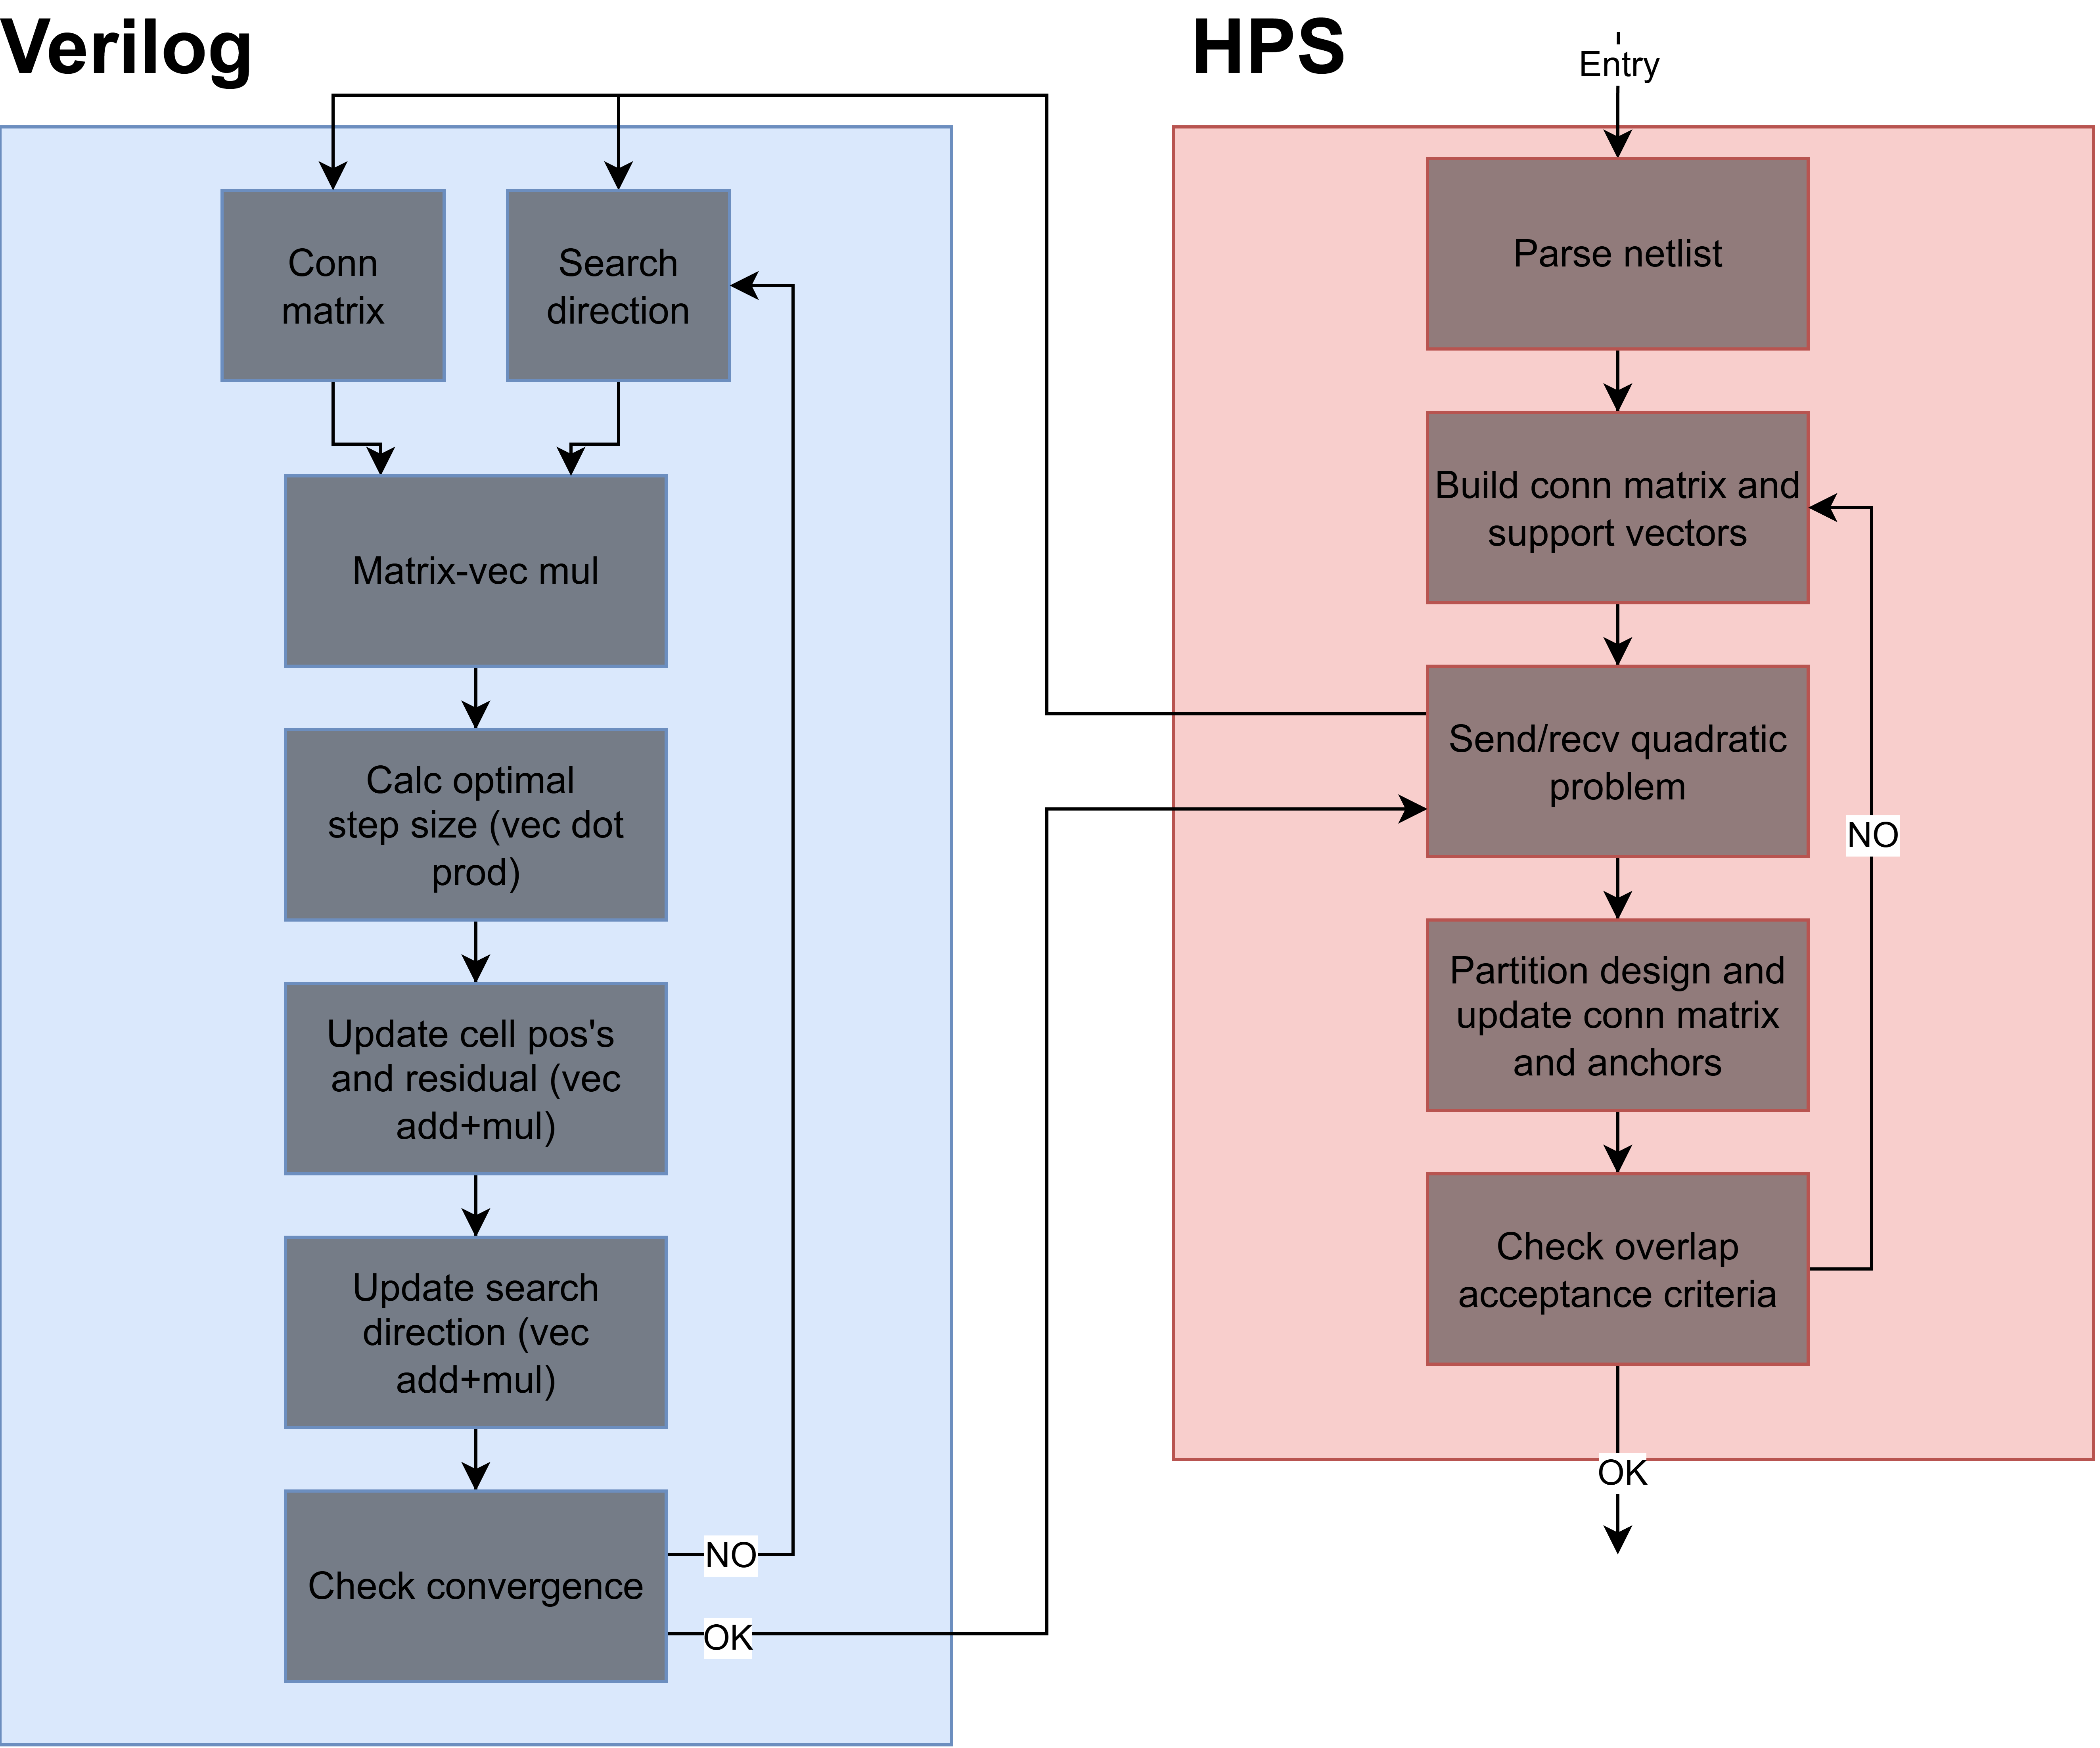
\includegraphics[width=0.45\textwidth]{ece5760-final-project-diagram.png}
    \caption{Block-level implementation of our analytical placer using a quadratic wirelength model with the clique net decomposition, partitioning-based overlap reduction, and fixed point integration. The HPS orchestrates the algorithm while the FPGA accelerates the conjugate gradient linear system solve.}
    \label{fig:overview}
\end{figure}

We will first write our pure-software placer entirely in C and run it on the DE1-SoC's ARM-based HPS. We will then offload the computational bottleneck---the conjugate gradient solve of the sparse linear system $Q\mathbf{x} = -\mathbf{c}$---onto the FPGA programmable logic. Specifically, the FPGA will implement a pipelined engine for the core CG operations: sparse matrix-vector multiplication, vector dot products, and scaled vector addition with the algorithm specified in Gundersen~\cite{gundersen2022conjugategradient} and shown graphically in Fig~\ref{fig:overview} and as pseudocode in Listing~\ref{lst:cgd}. As such, the HPS will remain responsible for algorithm orchestration: parsing the input netlist, constructing the connectivity matrix $Q$ and right-hand-side vector $\mathbf{c}$, creating the initial placement, performing the geometric bisection and generating anchor points, controlling the fixed-point iteration loop, and checking for convergence. The matrix and vector data will be communicated to the FPGA over the HPS-to-FPGA bridge, with results read back after each CG solve completes.

\begin{lstlisting}[caption={Conjugate Gradient Solve: $Q_x \mathbf{x} = -\mathbf{c}_x$}, label={lst:cgd}]
x  = x0
r  = -cx - Qx * x
d  = r
rr = dot(r, r)

for k = 1, 2, ... do
    q      = Qx * d
    alpha  = rr / dot(d, q)
    x      = x + alpha * d
    r      = r - alpha * q
    rr_new = dot(r, r)
    if rr_new < eps^2 then
        return x
    beta   = rr_new / rr
    d      = r + beta * d
    rr     = rr_new
end for
\end{lstlisting}

For input test cases, we plan to create a variety of benchmarks with varying numbers of cells, numbers of pins per net, and corner cases involving complex routes which lead to increased wirelength. Given the Cyclone V FPGA only has 390 M10K blocks of available SRAM, we will be limited in the size of the connectivity matrix we provide to it, and thus the number of cells we wish to place. If we wish to evaluate larger netlists, we will need to devise a streaming scheme to send data in real time to the FPGA.

We will verify our FPGA-based CG solver through simulation in Verilator and ModelSim before integrating it with the HPS to run the full algorithm pipeline. Our final results will compare the runtime of the pure-software HPS implementation against the HPS+FPGA accelerated version across multiple benchmarks, and we will report both HPWL and overlap metrics for each.

\section{AI Attribution}
We have used Claude for the initial explorations of this project by helping us find relevant papers on the topic, as well as understanding complex topics discussed in the paper. Claude has also helped us formulate a problem statement and our overall architecture based on our constraints including the CGD pseudocode. It also performed proofreading and technical checking of this proposal against our selected background information.

\bibliographystyle{IEEEtran}
\bibliography{references}

\end{document}